\section*{\begin{center}{\Huge Appendix A}\end{center}}
\addcontentsline{toc}{chapter}{Appendix A}
$\\[0.5cm]$

\section*{Artificial Neural Network Concepts}

% ===============================================================================
\subsection*{Formal Outline}
Mathematically speaking, ANNs may be outlined as follows;
\\
a network consists of a set $S$ of $N$ nodes. Furthermore, for every node $i\in S$: $i$ may be connected to a node $j \in S$.
\\
For every such connection, there exists a weight, $\omega_{i,j} \in \Re$, the sub-script denoting a connection weight from node $i$ to node $j$.
\\
A transfer function $f$ is a function $f(\theta)$ of a neuron's total input, $\theta$. A commonly used transfer function is the sigmoid transfer function, simply being 
\begin{equation}\label{sigmoid}
    f(\theta) = \frac{1}{1+e^{-\theta}}
\end{equation}
Neuronal activation $u_j$ of a node $j$ may be written as,

\begin{equation}\label{activation}
    u_j = f(\theta_j)
\end{equation}
where
\begin{equation}\label{input}
    \theta_j = \sum_{i\in M} u_i \omega_{i,j}
\end{equation}
and $M$ is the set of all nodes that have incoming connections to neuron $j$, $M \in S$, and $u_i$ is the activation value of node $i$. This is the principle which is used during the feed-forward phase in an FFBP ANN. In other words; the presented input is propagated throughout the network by calculating activation values for all nodes in the input layer, which then flows through the rest of the nodes in the network in the same manner until finally arriving at the output nodes.


% ===============================================================================
\subsection*{Back-propagation}\label{BP}

One way of updating the weights in an ANN is as previously mentioned by using back-propagation (BP) of an error signal. This may described as a fairly straight-forward algorithm for finding sub-optimal or optimal weights in an ANN. This is achieved by minimizing an error-signal which is back-propagated from the output node(s) of the network. Because the generation of an error signal requires an input pattern to be fed forward throughout a network, these two steps are commonly referred to together as feed-forward back-propagation (FFBP). Note, however, that the algorithm does not guarantee convergence towards a global optimum, as it is a gradient-based method, which traverses the weight space constituted by minimizing an error signal for a neural network. See figure \ref{fig:steepest_descent} for an illustration of this. An analogy to the problem of convergence towards a local optimum is simulated annealing, which runs the risk of being stuck in a local optimum of the temperature cools down too quickly. However, with just enough temperature and movement, or "jiggle", the algorithm may be able to continue its traversal, possibly finding a more optimal solution.

Mathematically, the back-propagate algorithm requires us to be able to calculate a gradient $\Delta \omega$ for each weight $\omega \in \Omega$, where $\Omega$ is the weight space for the network. Arriving at a given output for a given FFBP ANN through feed-forward propagation using the equations \eqref{sigmoid}, \eqref{input}, \eqref{activation}, the squared error may be expressed as,

\begin{equation}
    \textbf{E} = \frac{(\textbf{d} - \textbf{o})^2}{2},
\end{equation}
where $\textbf{d}$ is the desired output vector for all output nodes. Dividing by two to account for using two data points in finding the squared error.

This may then be used to calculate a gradient that may be used in updating every weight between the output layer and the preceding layer in the ANN,

\begin{equation}\label{weight_update}
    \omega_{t+1}^{i,j} = \omega_{t}^{i,j} + \Delta \omega_{t}^{i,j},
\end{equation}

In order to perform a weight change in the direction of minimizing the error loss function $\textbf{E}$, the partial derivative of $\textbf{E}$ w.r.t. the weight $\omega_{i,j}$ is used,

\begin{equation}
    \Delta \omega_{i,j} = -\alpha \frac{\partial \textbf{E}}{\partial \omega_{i,j}},
\end{equation}

where $\alpha$ is a learning rate parameter. Note that the sub-script denoting time is dropped for convenience.
The negative is used in order to adjust for the error. Despite the fact that BP does not guarantee convergence towards the global optimum (here minimum), it can be shown that for a sufficiently fine-grained step-parameter (i.e. learning rate), convergence towards a local optimum can be guaranteed. This is due to the nature of the search space, which is continuous and differentiable, but may contain ridges and local minima in terms of the squared error, $\textbf{E}$. However, the smaller the learning rate $\alpha$, the slower the convergence. Furthermore, for too low an $\alpha$, the gradient's "reach" will also decrease, making it more prone to small stationary points in the weight space. In other words, a learning rate parameter which will converge at a "fair" rate towards the optimum is preferable. This rate is domain specific. Illustratively, if $\alpha$ is too large, the algorithm is chaotic, resulting in divergence when using gradient descent in weight space. If it is too small, the algorithm is very stable and unable to traverse large parts of the weight space. Lastly, if $\alpha$ is of a preferable size, the algorithm is at the edge of chaos - able to traverse larger parts of the weight space, yet eventually converging towards a solution. See figure \ref{fig:steepest_descent} for an illustration of this.

Using the chain rule, one may obtain the weight change update in a given layer as (see below in chapter \ref{bptt-derivation} for a derivation),

\begin{equation}\label{recursive_derivative_error_activation_input}
    \frac{\partial \textbf{E}}{\partial u_j}\frac{\partial u_j}{\partial \theta_j} = 
    (\sum_{l \in L}\frac{\textbf{E}}{\partial u_l}\frac{\partial u_l}{\partial \theta_l}) f(\theta_j)(1-f(\theta_j),
\end{equation}

which accounts for the weight change updates of the preceding layers too, the first layer being,

\begin{center}
\begin{math}
    \frac{\partial \textbf{E}}{\partial u_l} \frac{\partial u_l}{\partial \theta_l} \omega_{j,l} = 
    u_l (u_l - d_l) \omega_{j,l},
\end{math}
\end{center}
Making it possible to obtain the partial derivatives recursively by starting at the output layer and back-propagating the values into the partial derivatives for $\textbf{E}$ for every weight $\omega_{i,j}$.

\begin{figure}
\centering
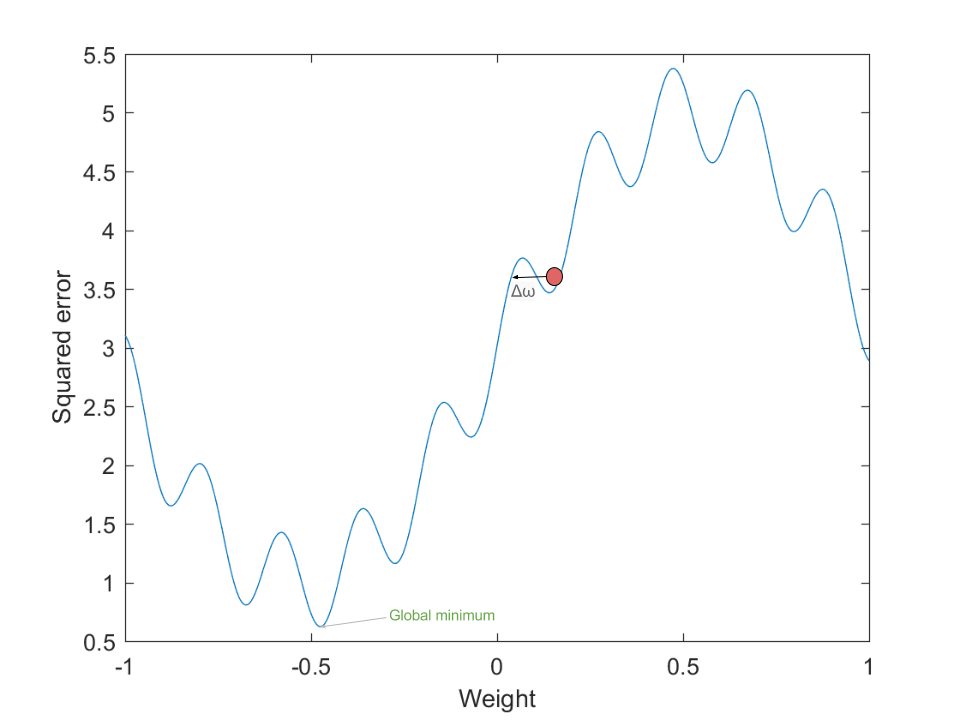
\includegraphics[width=10cm]{fig/error_landscape_with_ball.png}
\caption{Illustrating the error-landscape formed by finding the weights in an ANN that minimize the sum of squared errors, shown for one particular weight and its associated squared error. When traversing the landscape formed by $\textbf{E}$, local minima may be encountered (in between ridges). An analogy which is often used in illustrating this is a ball rolling down the hills because of kinetic energy imposed on it by gravity. In this analogy $\alpha$ would in a sense be friction, constraining the work of gravity and resulting in a smaller or larger velocity, i.e. step sizes $\Delta \omega$ for each iteration of the algorithm.
Too small an acceleration may result in the ball stopping when encountering a ridge. In the event of this being a local minimum, we would of course prefer for the ball to have enough kinetic energy to traverse the ridge and fall into a lower valley. Therefore, just enough acceleration to traverse the local minima is preferable. However, using too high an acceleration, the ball might not settle into any attractor at all. Possibly the weights will even diverge, with the ball being launched into outer space, sealing its fate to never again return to the hillside.}
\label{fig:steepest_descent}
\end{figure}

\begin{figure}
\centering
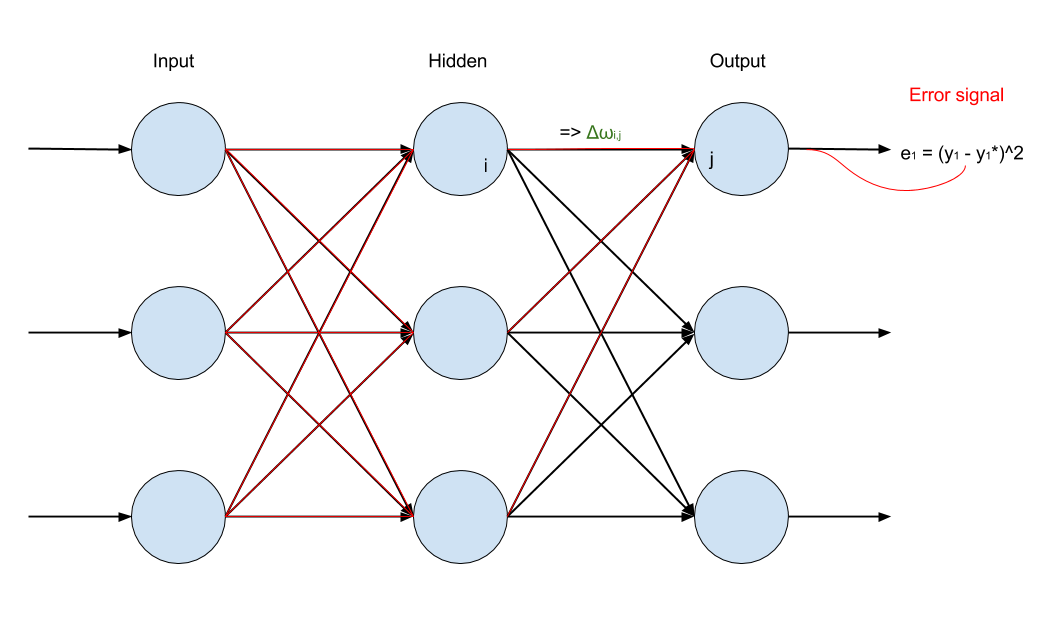
\includegraphics[width=13cm]{fig/BP_error}
\caption{Illustrating the back-propagation of an error-signal, with the error signal from every output node having an impact on the resulting weight gradient that is calculated for every weight in the network. Note that the red lines are the lines symbolize the propagation of the error signal from output node $j$ to all of its predecessors. $y_1$ is the obtained output, whereas $y_1^*$ is the desired output, and $e_1$ is the squared error for the output node.}
\label{fig:BP_error}
\end{figure}

% ====================================
\subsubsection{Back-propagation Through Time}

The algorithm of section \ref{BP} may be extended by taking into account the $k$ last time-steps of training in a network. Implementations may vary, the key here being a time-dependence. By introducing a measure which averages over the former weights, it turns out that convergence may be faster than when only using BP (as opposed to here BPTT). An alternative approach is to include $k$, or all previous weights, discounting the impact each former weight has exponentially as a function of time.

\begin{center}
\begin{math}
    \omega_{t+1} = \sum_{i=0}^{k}\gamma^i \omega_{t-i},
    \gamma \in (0, 1)
\end{math}
\end{center}


% =============================================================================================
\section*{Derivation of the Back-propagation Rule}\label{bptt-derivation}

The following derivation is based primarily on the derivation of \cite{Rumelhart1986}, as well as on that of \cite{Russell2009}.
Using the chain rule, one may formally derive $\Delta \omega$ the following way,

\begin{equation}
    \frac{\partial \textbf{E}}{\partial \omega_{i,j}} = \frac{\partial \textbf{E}}{\partial u_j}
    \frac{u_j}{\theta_{j}}
    \frac{\theta_{j}}{\omega_{i,j}},
\end{equation}
where the partial derivative w.r.t. the weight between nodes $i$ and $j$ will be cancelled out for all nodes other than $j$. Formally,

\begin{center}
\begin{math}
    \frac{\partial \theta_j}{\partial \omega_{i,j}} = \frac{\partial}{\partial \omega_{i,j}}(\sum_{k \in M}{} \omega_{k,j}o_k),
\end{math}
\end{center}

\begin{center}
\begin{math}
    \frac{\partial \omega_{k,j}o_k}{\partial \omega_{i,j}} = 0 : k \neq i,
    \implies
\end{math}
\end{center}
\begin{equation}
    \frac{\partial \theta_j}{\partial \omega_{i,j}} = u_i.
\end{equation}

\begin{equation}
    \frac{\partial u_j}{\partial \theta_j} = \frac{\partial}{\partial \theta_j} f(\theta_j) = f(\theta_j)(1-f(\theta_j))
\end{equation}

\begin{equation}
    \frac{\partial \textbf{E}}{\partial u_j} = \sum_{l \in L}(\frac{\partial \textbf{E}}{\partial \theta_l} 
    \frac{\partial \theta_l}{\partial u_j})
    = \sum_{l \in L}(\frac{\partial \textbf{E}}{\partial u_l} \frac{\partial u_l}{\partial \theta_l} \omega_{j,l}),
\end{equation}
where $L$ is all nodes to which node $j$ is connected - i.e. the set of nodes with \textit{outgoing} links from $j$. From this it can be seen that when $l$ is an output node,

\begin{center}
\begin{math}
    \frac{\partial \textbf{E}}{\partial u_l} \frac{\partial u_l}{\partial \theta_l} \omega_{j,l} = 
    u_l (u_l - d_l) \omega_{j,l},
\end{math}
\end{center}
Making it possible to obtain the partial derivatives recursively by starting at the output layer and, surprisingly, back-propagating the values into the partial derivatives for $\textbf{E}$ for every weight $\omega_{i,j}$.

In other words, the weight change update in a given layer accounts for the weight change updates of the preceding layers too. Formally,

\begin{equation}
    \frac{\partial \textbf{E}}{\partial u_j}\frac{\partial u_j}{\partial \theta_j} = 
    (\sum_{l \in L}\frac{\textbf{E}}{\partial u_l}\frac{\partial u_l}{\partial \theta_l}) f(\theta_j)(1-f(\theta_j).
\end{equation}

% =============================================================================================
\section*{The Vector L2-norm}\label{l2-norm}

For a vector
\begin{math}
    \textbf{v} = \begin{bmatrix} x_1 & x_2 & ... & x_n
        \end{bmatrix}^T,
\end{math}
the l$^2$-norm of the vector is defined as,

\begin{equation}
    |\textbf{v}| = \sqrt{\sum_{i=1}^{n} x_i^2},
\end{equation}
for real-valued vectors. [ref. the bible]

\cleardoublepage